\documentclass[12pt]{article}
\usepackage[utf8]{inputenc} % uft8 you know
\usepackage[danish]{babel}
\usepackage{lastpage}
\usepackage{fancyhdr}
\usepackage{hyperref}
%\usepackage{biblatex}
\usepackage[T1]{fontenc}
\usepackage{ae}
\usepackage{graphicx}
%\usepackage{pdfpages} % Til at inkludere pdf'er
\usepackage{amsmath}
\usepackage{amsfonts}
\usepackage{amssymb}
\usepackage{adjustbox}
\usepackage{blindtext}
\usepackage{geometry}
\usepackage{tabularx, booktabs, siunitx}
\usepackage{multirow}
\usepackage{titlesec}
\usepackage{longtable}
\usepackage[margin=0.2cm]{caption}
\titleformat{\section}
{\normalfont\Large\bfseries}{\thesection}{1em}{}
\titleformat{\subsection}
{\normalfont\large\bfseries}{\thesubsection}{1em}{}
\titleformat{\subsubsection}
{\normalfont\normalsize\bfseries}{\thesubsubsection}{1em}{}
\titleformat{\paragraph}[runin]
{\normalfont\normalsize\bfseries}{\theparagraph}{1em}{}
\titleformat{\subparagraph}[runin]
{\normalfont\normalsize\bfseries}{\thesubparagraph}{1em}{}
\usepackage{natbib} % Works with.bib files
\bibliographystyle{apalike} 


\geometry{
    a4paper,
    total={170mm,257mm},
    left=20mm,
    top=20mm,
    bottom=30mm,
}
\hypersetup{
    linkcolor=black,
    colorlinks=false,
    pdftitle={Biologi eksammen - af Kristoffer Sørensen},
    pdfauthor={Kristoffer Sørensen},
    % Remove the red border around links
    pdfborder={0 0 0},
}

\pagestyle{fancy} % definds the pagestyleing
\fancyhf{} % Removes the wired header text
\renewcommand{\headrulewidth}{0pt} % Removes the line under the header
\cfoot{Side \thepage\ af \pageref{LastPage}} % Sets the right side of the footer to "Page X of Y"
%\lhead{Gruppe 1} % Sets the left side of the header to "Gruppe 1"

\begin{document}
    %\providecommand\NAT
    \title{
    DIO - Atombomben \\ 
    \large{Rybners HTX - Vejleder: PJE og DP} \\
    \small{Idehistorie B og Dansk A}
}
\author{Af Kristoffer Sørensen}
\thispagestyle{empty}
\maketitle
\begin{figure}[h!]
    \centering
    
\includegraphics[width=0.9\textwidth]{figurs/forsideimg.jpg}
    \caption{Nuclear Bomb Explosion - Mushroom Cloud stock photo (\cite{RomoloTavani2018}) }%\cite{Forsideimg}} TODO: Add source
    \label{fig:Forsideimg}
\end{figure}
\newpage

    % Alle spørgsmål vil få sin egen fil, som vil blive inkluderet her.
    \newpage
\part{Celletyper og deres organeller}\label{sec:celletyperogderesorganeller}
    \section*{Redegør for cellers opbygning, herunder forskelle og ligheder mellem forskellige celletyper.}
        For at kunne påpeje hvad forskellighederne mellem de forskellige celletyper er tror jeg at det er vigtit at man ved hvad de forskellige celle typer er. 
        Der finde 2 forskellige celletyper, som er:
        \begin{itemize}
            \item Prokaryote celler (Celler unden cellekernen)
            \item Eukaryote celler (Celler med Cellekernen)
        \end{itemize}
        Ganske kort så er forskellen på de 2 celletyper at prokaryote celler ikke har en cellekerne, hvorimod eukaryote celler har en cellekerne.
        \subsection*{Hvad er en Eukaryot celle?}
            Eukaryote celler kender vi fra utallige steder, da det er de celler som vi finder i planter og dyr, Herunder også mennesker.
            De eukaryote celler indeholder som sagt en cellekerne. De er forholdsvis store, og er afgrænset af en cellemembran. 
            Et overall navn for alt der er i en celle undtagen cellekerne er cytoplasma. Cytoplasma er den del af cellen som indeholder alle organellerne, såsom mitokondrier, ribosomer, og mange flere.
            \paragraph{Cellekernen (nucleus)}
                Cellekernen er en af de vigtigste organeller i en celle. I mennesket celler er der 46 kromosomer, og 23 kromosom-par. Hvert kromosom, indeholder et DNA-mollekyle og særlige proteiner.(Se mere her\ref{sec:protein}).
                Cellekernen, også kendt som nucleus, er en af de mest fundamentale komponenter i en celle. Den er en organell, som er omgivet af en dobbeltmembran og indeholder det meste af cellens genetiske materiale. Her er nogle af de vigtigste karakteristika ved cellekernen:

                Genetisk materiale: Cellekernen indeholder det meste af cellens DNA, som er organiseret i strukturer kendt som kromosomer. DNA indeholder genetisk information, der er nødvendig for at kontrollere cellefunktioner og arvelighed.

                DNA-replikation og transkription: Cellekernen er stedet for DNA-replikation (kopiering af DNA før celledeling) og transkription (processen, hvor en del af DNA-sekvensen kopieres til mRNA, som derefter bruges til at lave proteiner).

                Regulering af genekspression: Cellekernen spiller også en central rolle i reguleringen af genekspression, det vil sige processen, hvor information fra et gen bruges til at lave et funktionelt produkt, typisk et protein.

                Beskyttelse af genetisk materiale: Ved at indeholde DNA i en adskilt struktur, beskytter cellekernen DNA fra potentielle skader, der kunne forekomme i cytoplasma.

                Det er vigtigt at bemærke, at ikke alle celler har en cellekerne. For eksempel har bakterier ikke en cellekerne; i stedet er deres DNA fritflydende i cellen. Dette er en af de vigtigste forskelle mellem prokaryote (uden cellekerne) og eukaryote (med cellekerne) celler.
                
            \paragraph{Mitokondrier}
                En ting som prokaryote celler heller ikke har er Mitokondrier. Det har en eukaryote celle dog. Mitokondrier er et organell som står for at danne ATP.
                ATP er et molekyle som indeholder kemisk energi, som cellen kan bruge til at udføre arbejde. Behovet for ATP er meget stort, da det er med til at drive mange af cellernes processer, herunder celledeling.   
            
        \subsection*{forskelle og ligheder mellem planteceller og dyre celler}
            En eukaryote celle er som før nævnt en celle som har en cellekerne, og ses ved blandt andre Dyre celler og planteceller. Men hvad er forskellen på en dyre celle og en plantecelle, og hvad har de tilfældes?
            \newline\textbf{Ligheder mellem planteceller og dyreceller:}\newline
            Cellekernen: Begge har en cellekerne, der indeholder cellens DNA.
            Organeller: Begge indeholder organeller, såsom mitokondrier, endoplasmatisk reticulum, og Golgi-apparatet.

            Cytoplasma: Begge indeholder cytoplasma, en geléagtig substans, der fylder cellen og indeholder organellerne.

            Cellemembran: Begge har en cellemembran, der styrer, hvilke stoffer der kan komme ind og ud af cellen. \\
            \textbf{Forskelle mellem planteceller og dyreceller:}\newline

            Cellevæg: Planteceller har en cellevæg lavet af cellulose, der giver ekstra struktur og støtte. Dyreceller har ikke en cellevæg.

            Kloroplaster: Planteceller indeholder kloroplaster, hvor fotosyntese foregår for at producere glucose. Dyreceller har ikke kloroplaster, da de ikke udfører fotosyntese.

            Store central vakuole: Planteceller indeholder en stor central vakuole, der lagrer vand og hjælper med at opretholde celleturgor. Selvom dyreceller også kan have vakuoler, er de generelt mindre og ikke så fremtrædende som i planteceller.

            Cytoskelet og centrosomer: Dyreceller har centrosomer, der hjælper med celledeling, mens de fleste planteceller ikke har. Desuden er dyrecellers cytoskelet mere udtalt og komplekst end det hos planteceller.

    \subsection*{Redegør for cellernes forskellige organeller samt deres funktion. Kom herunder ind på fotosyntese og respiration.}
        Eukaryote celler, der er til stede i planter, dyr, svampe og protister, rummer en række specialiserede organeller, hver med sine unikke funktioner. Lad os dykke ned i nogle af de mest markante organeller og deres roller:

        I planteceller finder man organeller kaldet kloroplaster. Kloroplaster er ansvarlige for fotosyntesen, en proces, der konverterer lysenergi til kemisk energi. Da fotosyntese ikke forekommer i dyreceller, er disse celler uden kloroplaster.
        
        Både planteceller og dyreceller indeholder mitokondrier, som er centrale for produktionen af ATP. ATP, eller adenosintrifosfat, er et molekyle, der indeholder kemisk energi, som cellen kan bruge til at drive forskellige processer. ATP's rolle er vital, idet det driver mange af cellens processer, herunder celledeling.
        
        Men hvordan produceres ATP? Svaret ligger i en proces kaldet respiration. Respiration er en biologisk proces, hvor celler nedbryder glukose for at frigive energi, som de kan bruge. Der er to hovedtyper af respiration: aerob og anaerob.
        
        Aerob respiration, der kræver ilt, er en mere effektiv proces sammenlignet med anaerob respiration. Det er fordi aerob respiration producerer omkring 36 ATP-molekyler, mens anaerob respiration, der kan forekomme uden ilt, kun producerer 2 ATP-molekyler. En anden forskel er, at anaerob respiration resulterer i produktionen af mælkesyre, mens aerob respiration ikke gør det. Desuden forekommer anaerob respiration i cytoplasmaet, mens aerob respiration hovedsageligt forekommer i mitokondrierne. \\
        \textbf{Cellulær Respiration: (Cellulær respiration kan være både aerob og anaerob) }\begin{equation}C_6H_{12}O_6 + 6CO_2 \rightarrow 6O_2 + 6H_2O + ATP \end{equation}


    \subsection*{Diskuter forsøget om papirchromatografi, og kom i den forbindelse ind på betydningen af fotosyntese og respiration, i organismen, såvel som i et økosystem}
        % TODO: Skriv om papirchromatografi
        

    \subsection*{Yderlige informationer om Celler og organeller}
    Hvordan er det nu med de proteiner i DNA-mollekylet? \label{sec:protein} En DNA-streng er indpakket omkring otte histonproteiner for at danne en struktur kaldet en "nukleosom". En serie af nukleosomer, der ligner perler på en snor, snoes og foldes for at danne en mere kompleks struktur kaldet kromatin. 

    \newpage
\section{Transport ind og ud af celler}
    \subsection{Redegør for opbygningen af celler. Herunder deres organeller samt transport ind og ud af cellen.}
        For at læse omkring celler henvises til \textbf{Kapitel 1: Celler} på side \pageref{sec:celletyperogderesorganeller}.
        \begin{center}
            \begin{longtable}{ | m{2cm} | m{11cm}| m{2cm} |}
                \caption{Transport-processer} \\
                \hline
                \textbf{Transport-proces} & \textbf{Hvordan fungere processen og hvilke stoffer transporteres på denne måde?} & \textbf{Aktiv eller pasivt}\\
                \hline
                Diffusion & Diffusion er en proces, der sker naturligt i naturen, hvor molekyler bevæger sig fra områder med høj koncentration til områder med lav koncentration. 
                Denne proces fortsætter, indtil der er ligevægt, det vil sige, at koncentrationen af molekyler er den samme overalt. Der er to hovedtyper af diffusion, der finder sted i celler: 
                simpel diffusion og faciliteret diffusion. \textbf{Simpel diffusion:}  ette er den grundlæggende form for diffusion, hvor molekylerne bevæger sig frit gennem cellemembranen uden brug af transportproteiner. 
                De molekyler, der typisk bevæger sig på denne måde, er små, ikke-polære molekyler, såsom oxygen og carbon dioxide. Vand kan også passere gennem membranen på denne måde via en proces kaldet osmose. Det kræver ingen energi (ATP) fra cellen, og derfor betegnes det som en passiv transportform. & Passiv\\
                \hline
                Osmose & Osmose er en specifik type af passiv transport, der er meget vigtig i biologiske systemer. Den involverer bevægelsen af vandmolekyler fra et område med lav solutkoncentration (høj vandkoncentration) til et område med høj solutkoncentration (lav vandkoncentration) gennem en semipermeabel membran.

                En semipermeabel membran er en type barriere, der tillader visse stoffer at passere igennem, men blokerer for andre. I tilfældet med osmose tillader den vand at passere igennem, men forhindrer mange andre molekyler, særlig store eller ladede molekyler, i at gøre det.
                
                Der er tre hovedtyper af osmotiske forhold:
                \textbf{Isotonisk: }  Her er koncentrationen af solut (opløst stof) den samme på begge sider af membranen. Der vil derfor ikke være nogen bevægelse af vand. 
                \textbf{Hypertonisk: } Her er koncentrationen af opløst stof højere uden for cellen end inden i den.
                Vand vil tendere til at bevæge sig ud af cellen for at fortynde soluten uden for cellen, hvilket kan forårsage cellen til at skrumpe.
                \textbf{Hypertonisk: } er er koncentrationen af opløst stof lavere uden for cellen end inden i den. Vand vil tendere til at bevæge sig ind i cellen for at fortynde oplæste stof inde i cellen, hvilket kan forårsage cellen til at svulme og potentielt briste. & Passiv\\
                \hline
                Aktiv transport & Aktiv transport er en proces hvor molekyler bevæger sig fra et område med lav koncentration til et område med høj koncentration. Større molekyler kan komme igemmen her. & Aktiv\\
                \hline
                Faciliteret diffusion & Faciliteret diffusion er en proces hvor molekyler bevæger sig fra et område med lav koncentration til et område med høj koncentration. Glukose kan blandes med vand og derfor være et polært stof. Og det har derfor ikke diffundere ved brug af simpel diffusion hen over en celle membran, da en cellemembran er lavet af Fosfolipider altså fedt stof. Derfor skal glukose bruge en transport protein for at komme igennem cellemembranen.  
                & Passiv\\
                \hline
            \end{longtable}
        \end{center}

    \subsection{Forklar forsøget: Osmose i kartofler.}
    \subsection{Diskuter hvordan transport over cellemembranen spiller en vigtig rolle for organismer.}
    \newpage
\part{Biokemiske processer}
    \section{Forklar de 2 biokemiske processer respiration og fotosyntese.}
        \subsection{Respiration}\label{sec:respiration}
            Hvad er Respiration? 
        \subsection{Fotosyntese}
            I en eukaryot plantecelle har man et organell som man ikke har i en eukaryot dyre celle, nemlig grønkorn. I grønkornene sker der en masse biokemiske processer som vi tilsammen kalder for fotosyntese. Under fotosyntese dannes to vigigtige stoffer, nemlig glucose og ilt. glucose (\begin{math}C_6H_{12}O_6\end{math}) er en sukkerart som er vigtig for planten, da den bruger den til at danne andre stoffer som den har brug for. 
            \begin{math}O_2\end{math} er ilt, som er vigtigt for alle levende organismer, da det er det vi bruger til at danne energi her i blandt \ref{sec:respiration}.
            I fotosyntese skal planten bruge to ting \begin{math}CO_2\end{math} og \begin{math}H_2O\end{math}. Alt det førnævte er ting som planten optager fra det miljø den er i. De to stoffer bruges til at skabe det organiske stof glucose. Glucose er et meget energirigt stof derfor kræve fotosyntese lysenergi. Heraf foto-syntese (lys drevet syntese)  \begin{math}H_2O\end{math} er vand, som planten optager fra jorden.
            Den simple formel for fotosyntese er: \begin{equation} 6CO_2 + 6H_2O \rightarrow C_6H_{12}O_6 + 6O_2 \end{equation}\label{eq:fotosyntese}
            Fotosyntese består af de 15-20 delprocesser, som overall kan beskrives med den fromel som ses ovenfor. (Se afsnit \ref{eq:fotosyntese})
            Man kan dele disse processer op i to dele hhv mørke- og lysprocessen. \newline 
            \subsubsection{Lysprocessen}
                Lys processerne kræver lys og kan kun foregå når der er lys til stede. Lysprocessen sker i thylakoiderne. I processen bliver der brugt \begin{math}H_2O\end{math} O som bliver lavet om til ilt og hydrogen. Hydrogen bliver hoverført til \begin{math}NADP^+\end{math} så det danner \begin{math}NADPH\end{math} (\begin{math}NADPH\end{math} er et organiske molekyle.) 
                Lysenergien anvendes til at sammensætte \begin{math}ADP + P_i\end{math} Og på den måde omdannes \begin{math}ADP\end{math} og \begin{math}P_i\end{math} til \begin{math}ATP\end{math} Denne process er afhængig af chloroflyl (Det som absorbere lysenergien) under lysprocessen dannes altså \begin{math}ATP\end{math} og \begin{math}NADPH\end{math} og ilt. En del af ilten bruges til respiration (se afsnit \ref{sec:respiration}), mens resten af ilten frigives til atmosfæren.

            \subsubsection{Mørkeprocessen}
                Mørkeprocessen er den del af fotosyntesen som ikke kræver lys. Denne proces foregår i grønkornene. Denne proces er en meget kompleks proces, som vi ikke vil gå i dybden med. Det vi skal vide er at den bruger energi fra lysprocessen til at danne glukose.


    \section{Redegør for øvelsen: Fotosyntese og Respiration hos vandpest.}
    \section{Diskuter hvordan de 2 processer kan have indflydelse på klimaet.}
    \newpage
\part{Makromolekyler}
    \section{Redegør for opbygning af de makromolekyler der findes i fødevarer.}
        Der er 4 forskellige makromolekyler i fødevarer, nemlig kulhydrater, proteiner, fedtstoffer, og nukleinsyrer. Jeg vil mest komme ind på de 3 første. 
        \subsection*{Lipider (fedtstoffer)}
           Den normale måde at indtage fedt på er ved triglycerid. Fedt er vigigt for kroppen da det er en energi kilde. Fedt er også vigtigt for kroppen da det er med til at danne cellemembranen. Fedt er også med til at danne hormoner.
           Lipider er en bred klasse af biologiske molekyler, der er kendetegnet ved deres opløselighed i ikke-polar organiske opløsningsmidler og deres uopløselighed i vand. Lipider kan opdeles i forskellige undergrupper baseret på deres struktur, herunder triglycerider, fosfolipider, steroler og andre. Her er en kort beskrivelse af strukturen af nogle af de mest almindelige typer lipider:

           \textbf{Triglycerider:} Dette er den mest almindelige type lipid og den form, hvori kroppen opbevarer fedt. En triglycerid består af et glycerolmolekyle, der er bundet til tre fedtsyremolekyler. Fedtsyrer er lange kæder af carbon og hydrogen, der kan variere i længde. Fedtsyrerne kan være mættede (ingen dobbeltbindinger mellem carbonatomer) eller umættede (en eller flere dobbeltbindinger). Når vi taler om fedtsyrer, snakker man om "mættet" og "umættet" til strukturen af fedtsyrekæden, især til antallet af dobbeltbindinger mellem carbonatomerne i kæden.
           Mættede fedtsyrer: Mættede fedtsyrer har ingen dobbeltbindinger mellem carbonatomerne. Dette betyder, at hvert carbonatom er bundet til (eller "mættet med") det maksimale antal hydrogenatomer. Mættede fedtsyrer er typisk faste ved stuetemperatur og findes i animalske produkter som kød og mejeriprodukter, samt i nogle plantefødevarer som kokos- og palmeolie.
           
           Umættede fedtsyrer: Umættede fedtsyrer har en eller flere dobbeltbindinger mellem carbonatomerne. Dette betyder, at kæden ikke indeholder det maksimale antal hydrogenatomer - den er "umættet". Dobbeltbindingerne forårsager en knæk eller bøjning i fedtsyrekæden. Umættede fedtsyrer er typisk flydende ved stuetemperatur og findes i fødevarer som fiskeolie, olivenolie, rapsolie og nødder.
           
           Umættede fedtsyrer kan yderligere kategoriseres som "enkeltumættede" (hvis de har en dobbeltbinding) eller "flerumættede" (hvis de har mere end en dobbeltbinding). Omega-3 og omega-6 fedtsyrer, som du nævnte tidligere, er typer af flerumættede fedtsyrer.

            \textbf{Fosfolipider:} Fosfolipider er hovedkomponenten i cellemembraner. De har en struktur, der ligner triglycerider, men en af fedtsyrerne er erstattet med en fosfatgruppe. Dette gør en del af molekylet polært (og derfor vandopløseligt), mens resten af molekylet er nonpolært (og derfor uopløseligt i vand). Denne amfipatiske natur tillader fosfolipider at danne lipidbilag, som er grundlaget for cellemembraner.

            \textbf{Steroler:} \\ Steroler, som kolesterol, er en type lipid, der er kendetegnet ved en kompleks ringstruktur. Kolesterol er en vigtig komponent i cellemembraner, hvor det bidrager til fluiditet og stabilitet. Det er også forløberen for andre biologisk vigtige molekyler, herunder steroidhormoner, galdesalte og vitamin D.


            
        \subsection*{Kulhydrater - Sakarid}
        Mennesker har altid fået en stor del af deres energi i form af kulhydrater. Under fordøjelsen omdannes kulhydrater til glukose. Hjernens primære brændstof er glukose, og bl.a. derfor er kulhydrater en vigtig energikilde. I kulhydrater findes kulstof (C), brint (hydrogen (H)) og ilt (oxygen (O)) altid i forholdet 1:2:1. Derfor kan de almindeligste kulhydrater skrives efter Formlen: \begin{math}(CH_2O)_n\end{math}.
        Kulhydrater benævnes efter antallet af kulstofatomer i molekylet, hvorfor trioser, tetroser, pentoser og hexoser indeholder hhv. tre, fire, fem og seks kulstofatomer.
        Ernæringsmæssigt er det kun hexoserne, glukose og fruktose, der er interessante, fordi det er dem, der overvejende optages og omsættes i kroppen.
        Et kulhydratmolekyle kaldes et monosakkarid, når det ikke kan spaltes yderligere til et kulhydrat. Flere monosakkarider kan bindes til hinanden, hvorved der dannes kæder med eller uden forgrening. Disse kæder af monosakkarider inddeles efter, hvor mange monosakkarider som er bundet sammen. Således vil et disakkarid indeholde to monosakkarider, mens oligosakkarider og polysakkarider vil indeholde hhv. 3-9 og over 9 monosakkarider i molekylet. 
        \begin{figure}[h]
            \centering
            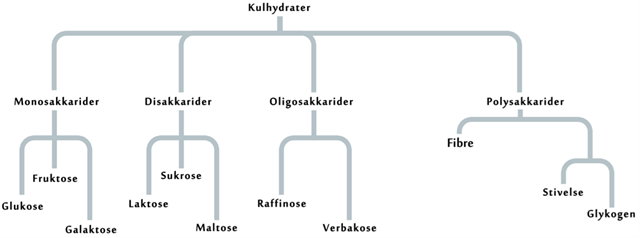
\includegraphics[width=0.8\textwidth]{figurs/carbs.png}
            \caption{Kulhydraterne inddeles i fire forskellige klasser afhængig af deres størrelse: monosakkarider, disakkarider, oligosakkarider og polysakkarider.}
            \label{fig:carbs}
        \end{figure}
        \begin{figure}
            \centering
            
\includegraphics[width=0.8\textwidth]{figurs/monosakarid.png}
            \caption{Monosakkarider}
            \label{fig:monosakkarider}
        \end{figure}
        \subsubsection*{Monosakkarider}
            De vigtigste monosakkarider i fødevarer og i organismen er glukose, fruktose og galaktose (figur \ref{fig:monosakkarider}); disse er alle hexoser. Fødevarer indeholder naturligt kun meget lidt af de tre monosakkarider (Se downloade tabel under eksammens mappe). Dog indeholder fx modne vindruer ca. 6,6 g fruktose og 6,8 g glukose pr. 100 g.
            I en vandig opløsning og i kropsvæskerne forekommer monosakkarider i både en lige kæde og i en ringform (figur \ref{fig:monosakkarider}) i forholdet 1:99. Det vil sige i en ligevægt, hvor 99 molekyler ud af 100 er på ringstruktur, og ét molekyle er på den lige form. Ringen dannes mellem C-atomet og iltatomet (O) i hhv. aldehyd- eller ketongruppen (figur \ref{fig:monosakkarider}). Monosakkariderne kan påvises og kvantitativt bestemmes vha. deres evne til at reagere med andre stoffer, der er betinget af indholdet af aldehyd eller ketongrupper. Især aldehydgruppen oxideres let til karboxylsyre. Den frie aldehydgruppe i glukose bevirker, at glukose kan reagere med protein. En kronisk forhøjet glukosekoncentration i blodet kan bevirke, at flere glukoseenheder bindes til proteiner, hvorved deres proteinstruktur og funktion ændres. Disse ændringer i proteinernes struktur ses hos nogle patienter med diabetes (sukkersyge).

            Monosakkarider kan også være pentoser, hvilket vil sige, de har fem kulstofatomer. I kroppen dannes pentoser primært ud fra hexosen glukose. Frie pentoser forekommer sjældent, men de er bestanddele af nukleinsyrerne i DNA (deoxyribonukleinsyre) i cellernes kerne (nucleus) og RNA (ribonukleinsyre). Pentoser findes desuden i ufordøjelige kulhydrater (kostfibre).


        \subsection*{Protein}
            Når man taler om at skulle have store guns så skal man have gains. Når man taler om gains taler man om både proteiner og kulhydrater. Men hvad er proteiner? Proteiner er et stort molekyle ligesom glucose. Proteiner er opbygget af aminosyre der findes 20 forskellige aminosyre som kan kombineres på utailige måder. Denne kæde af aminosyre kaldes også for et peptid. bindningerne mellem aminosyrerne kaldes for peptidbindinger. Læs mere om  peptidbindinger i afsnit \ref{fig:peptidbindinger}. Der findes 4 proteinstrukture
            \begin{itemize}
                \item Primærstruktur (1 - struktur)
                \item Sekundærstruktur (2 - struktur)
                \item Tertiærstruktur (3 - struktur)
                \item Kvartærstruktur (4 - struktur)
            \end{itemize}
            \textbf{Primærstruktur} er den struktur som er den simpleste.
            En normal kæde af aminosyre er primær, det der intificere at det er primærstruktur er at Den starter med \begin{math}NH_2\end{math} og slutter med en syregruppe \begin{math}COOH\end{math}.
            \textbf{Sekundærstruktur} er den stuktur som man kalder for Alpha helix og er den struktur som er foldet om sig selv som en spiral. Den Sekundærstruktur findes også som beta foldeblad. Beta foldebald er en slags siksak struktur. Der er også en beta vendning. Denne struktur binder de andre strukturer sammen.
            \textbf{Tertiærstruktur} er den rummelige opbygning af Beta foldebald, Beta vendning og Alpha helix. For at holde den rummelige opbygning sammen er der nogle svolvbroer. (cystein \begin{math}HS\end{math})
           \textbf{Kvartærstruktur} det er en samling af små proteiner det kunne være: Hemoplin, den består af 4 små proteiner. Altså protein kompleks som af flere mindre proteiner


\section{Hvilke funktioner har de forskellige makromolekyler i en organisme?}
Makromolekyler spiller en række forskellige roller i en organisme, afhængig af deres type:
    \subsection*{Proteiner}
        Proteiner fungerer som kroppens arbejdsheste, udfører de fleste af de cellulære processer, der holder en organisme i live. Proteiner kan handle som enzymer, der katalyserer kemiske reaktioner; som strukturelle komponenter, der giver celler og væv form; som transportmolekyler, der bærer stoffer rundt i kroppen; og som antistoffer, der bekæmper infektioner.

    \subsection*{Nukleinsyrer}
        Nukleinsyrer, herunder DNA og RNA, er ansvarlige for lagring og transmission af genetisk information. DNA lagrer den genetiske information, der bestemmer organismens egenskaber, mens RNA bruges til at oversætte denne information til proteiner.
    
    \subsection*{Kulhydrater}
        Kulhydrater tjener primært som energikilde for celler. Enkle sukkerarter, såsom glukose, kan bruges direkte til energi, mens komplekse kulhydrater, som stivelse og cellulose, kan lagre energi eller give struktur til celler og væv.
    \subsection*{Lipider}
        Lipider er involveret i en række forskellige funktioner, herunder energilagring, isolering, celledeling (som en del af cellemembranen) og signalering (som hormoner). For eksempel lagrer triglycerider energi, fosfolipider danner cellemembraner, og steroider fungerer som signalstoffer.

    Hver type makromolekyle spiller forskellige roller, men de arbejder alle sammen for at støtte livets processer i en organisme.
\section{Diskuter kostens betydning i forhold til sundhed. Inddrag øvelsen om kulhydrater i fødevarer}
    Kosten spiller en væsentlig rolle i forhold til sundhed. Her er nogle af de vigtige punkter, der understreger kostens betydning:

    Næringsstoffer: Den mad, vi spiser, forsyner vores krop med nødvendige næringsstoffer som proteiner, kulhydrater, fedt, vitaminer og mineraler. Disse næringsstoffer er nødvendige for kroppens forskellige funktioner, herunder energiproduktion, vævsvækst og reparation, og immunfunktion.

    Vægtkontrol: En afbalanceret kost hjælper med at vedligeholde en sund vægt. Overvægt og fedme, som ofte er resultatet af en usund kost, kan føre til forskellige sundhedsproblemer, herunder hjertesygdomme, type 2-diabetes og visse typer kræft.

    Sygdomsforebyggelse: En sund kost kan hjælpe med at forebygge visse sygdomme. For eksempel kan et kosthøjt i frugt og grønt, fuldkorn og magre proteiner hjælpe med at forebygge hjertesygdomme. En kost lav på sukker og mættet fedt kan hjælpe med at forebygge type 2-diabetes.

    Knoglesundhed: Indtagelse af nok calcium og D-vitamin i kosten er afgørende for knoglesundheden.

    Fordøjelsessystemets sundhed: En kost rig på fiber kan hjælpe med at forbedre fordøjelsessystemets sundhed ved at forebygge forstoppelse og reducere risikoen for visse sygdomme som tyktarmskræft.

    Mental sundhed: Nogle undersøgelser tyder på, at visse næringsstoffer som omega-3 fedtsyrer kan bidrage til mental sundhed ved at reducere symptomer på depression og angst.

    Selvom kosten er et centralt element i at opretholde en god sundhed, er det vigtigt at huske, at andre livsstilsfaktorer, som regelmæssig motion, tilstrækkelig søvn og undgåelse af tobak og overdreven alkohol, også er afgørende for vores overordnede velvære.
\section{Mere info}
\begin{figure}[h]
    \centering
    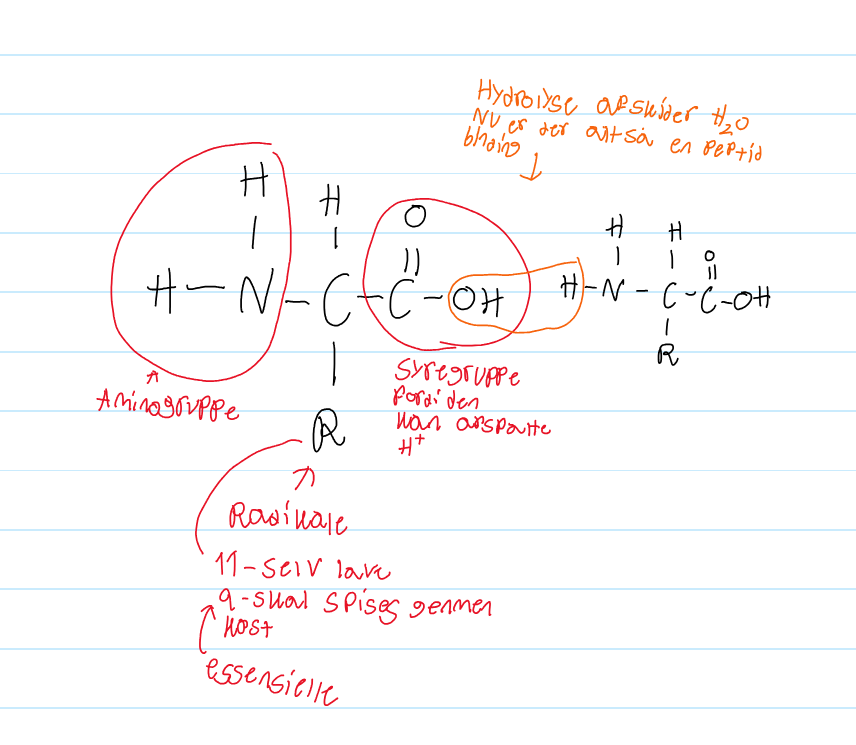
\includegraphics[width=0.8\textwidth]{figurs/peptidbindinger.png}
    \caption{Peptidbindinger}
    \label{fig:peptidbindinger}
\end{figure}
    \newpage
\section{Fordøjelse}
\subsection{Redegør for fordøjelsessystemets opbygning og funktion.}
\subsection{Forklar øvelsen: Bromelin i Ananas og relater til fordøjelsessystemet.}
\subsection{Diskuter hvordan blodsukker reguleres, og hvilke konsekvenser Diabetes kan have for mennesker.}
    \newpage
\part{Hormonregulering hos kvinder}
\subsection*{Forklar opbygningen og funktionen af de kvindelige kønsorganer}
\subsection*{Redegør for hvad hormoner er samt hvordan de transporteres og reguleres i kroppen.}
\subsection*{I forhold til øvelsen om prævention og sexuelt overførte sygdomme ønskes en redegørelse for præventions virkemåde. Kom desuden ind på fejlkilder i forsøget}
Både mænd og kvinder har mange forskellige kønsorganer med forskellige funktioner. Hos kvinder er der 13 forskellige kønsorganer, som har forskellige formål i kroppen. Klitoris, hymen, store kønslæber, små kønslæber, æggeledertragt, æggeleder, æggestok, livmor, livmorhals, blære, kønsben, urinrør og skeden. Klitorisen er ligesom penishovedet på den måde at den er tæt pakket med nerveceller, og kan derfor reagerer på lette berøringer. Skeden er klædt med en slimehinde og selve væggen er elastisk, når en kvinde indgår i samleje bliver der udskillet en væske som fungerer som et smøremiddel. Slimhinden producerer et kulhydrat som fremmer væksten af nogle mælkesyrerbakterier. De bliver brugt til at sørge for at uønskede bakterier ikke kan overleve i det sure miljø der er i skeden. Det primære kønsorgan for kvinder er æggestokkene, da det er der hvor æggene er anlagt. Ægcellerne liger i små væskefyldte blære som kaldes follikler. Hver måned bliver der modnet mange af æggene, dog er der typisk kun et æg der udvikles langt nok til at blive frigjort. Ægget samles op af æggeledertragten og føres hen mod æggelederen. I æggelederen vil ægget blive befrugtet og fortsætte mod livmoren, hvor det vil sætte sig fast i livmorvæggen. 
Cyklussen starter under puberteten og vil forsætte i 35-40 år efter. Som sagt sker der en modning af ægcellerne hver måned i folliklerne. Det sker da FSH for ægcellen til at vokse, og FSH stimulerer også follikelcellerne til at producere østrogen. Efter 14 dage vil der som regel kun være en follikel der er færdigudviklet og klar til ægløsning. Ægløsningen sker 14 dage efter der går hul på folliklen og det modne æg bliver frigivet. Ægget bliver frigjort når folliklen bliver stimuleret af LH, og på samme tid bliver follikelcellerne omdannet til det gule legeme hvor progesteron bliver dannet. Dog hvis ægget ikke bliver befrugtet så vil det gule legeme holde op med at fungere og menstruationen udløses.




Hormoner er stoffer der er nødvendige for en organisme, da de lader celler kommunikere med hinanden. Hormoner er som sagt stoffer, som bliver udskillet af specielle celler, og bliver brugt til at kommunikere med andre celler, der kan genkende hormonet. Celler kan genkende hormoner ved brug af hormon-receptorer. Hormoner bliver typisk lavet af endokrine kirtler, og hormoner bliver udskillet til blodbanen. Hos både mænd og kvinder bliver kønshormonerne primært udskillet fra kønskirtlerne, og selve reguleringen af hormonerne foregår mellem hypothalamus, hypofysen og kønskirtlerne. 
Det primære hormon hos kvinder er østrogen, dog er det ikke det eneste hormon kvinder danner, og bliver dannet på cirka samme måde som testosteron bliver dannet. Processen starter i hypothalamus hvor der bliver udskillet GnRH, som stimulerer hypofysen så der bliver dannet LH og FSH. FSH bliver brugt til at stimulerer æggestokkene, specifikt det gule legeme, så de kan danne østrogen og LH bliver også brugt til at stimulerer æggestokkene, dog så de kan danne progesteron. Ligesom hos mænd bliver koncentrationen af de primære hormoner reguleret ved brug af et negativt feedback loop. Når der er en høj koncentration af progesteron og østrogen i blodet vil hypofysens evne til at danne FSH og LH formindske. Faldet af koncentration af LH gør så det gule legemer henfalder, som fører til et fald i koncentrationen af østrogen og progesteron. Det betyder så også at hele processen kan ske igen da hypofysen kan igen begynde at danne LH og FSH til at stimulere æggestokkene og danne østrogen og progesteron igen.

I øvelsen om prævention og sexuelt overførte sygdomme skulle vi se hvordan kønssygdomme spreder sig og om præventionsmiddler hjælper med at stoppe spredningen af kønssygdomme. Vi brugt reagensglas som en erstatning af penissen. Kondom som vores præventionsmiddel, petriskåle med agar for at vi kunne tydeligt se hvor bakterierne spredte sig. Vi brugte også E.Coli som en erstatning af klamydia da det ikke ville have været sikkert for os at lege med en kønssygdom. Min gruppe kom dog til at lave fejl under forsøget da vores resultater gik helt imod alle andre gruppers. Den første fejl vi lavede var at vi pressede reagensglasset alt for hårdt mod agaren i petriskålene. Det gjorde så det var svært for os at aflæse resultaterne og har måske også revet hul i kondomen, hvilket er et selvfølge at det er en fejl, da forsøget handlede om præventionsmidler. Vi glemte også at tage stilling for at det kun var E.Colien der kom ind i petriskålene og vi regner med at der også har været noget kontaminering fra kimnedfald som har forvrænget vores resultater. 
Vi ved dog at en kondom burde fungere ved at sikre sig at der er ingen kontakt mellem det mandlige kønsorgan og andre steder. Det burde stoppe spredningen af kønssygdomme da det fungerer som en barriere og stoppe en overførelse af kropsvæsker mellem partnere. Dog er det jo ikke det eneste kondommer bliver brugt til da det også virker som en måde at forhindre gravidtitet, ved at, som sagt, forhindre at sæd bliver overført fra penissen til skeden.


    \newpage
\section{Hormonregulering hos mænd}
\subsection{Forklar opbygningen og funktionen af de mandlige kønsorganer}
\subsection{Redegør for hvad hormoner er samt hvordan de transporteres og reguleres i kroppen.}
\subsection{I forhold til øvelsen om prævention og sexuelt overførte sygdomme ønskes en redegørelse for præventions virkemåde. Kom desuden ind på fejlkilder i forsøget}
    \newpage
\part{Organer og kredsløb}
\subsection*{Forklar kort om nogle udvalgte organsystemer. Kom ind på deres funktion}
\subsection*{Redegør for kredsløbets opbygning og funktion, med særligt fokus på det lille kredsløb}
\subsection*{I forhold til øvelsen: fysiologiske målinger (puls, blodtryk, fedtprocent, BMI og vitalkapacitet) ønskes en diskussion om hvordan motion spiller en rolle for sundhed.}
En organisme kan opdeles i en masse forskellige organsystemer, der har forskellige formål, integumentære system, skelettet, muskelsystemet, nervesystemet, endokrinsystemet, cardiovaskulære system, lymfesystemet, respirationssystemet, fordøjelsessystemet, urinvejssystemet, immunsystem og forplantningssystemet. 
Nervesystemet er det system der står for at regulere og koordinere forskellige aktiviter i kroppen. Selve systemet består af tre mindre systemer: Det centrale system, det perifere system og det autonome nervesystem. Det centrale nervesystem består af rygmarven og hjernen, begge af dem er lavet af nerveceller og nervefibre. Det centrale nervesystem står for at sende nerveimpulser fra hjernen hen til rygmarven hvor det så bliver sendt videre til det perifere system. Det perifere system er nerverne som fører impulserne fra hjernen og rygmarven hen til resten af kroppen. Det står også for at få sendt impulser fra resten af kroppen til rygmarven og derefter til hjernen så det er muligt for hjernen at kommunikere med musklerne. Det autonome nervesystem er et system som vi ikke kan kontrollerer bevidst. Det står for at kontrollerer kropstemperatur, puls, indre organer osv. 
Fordøjelsessystemet er det system der står for at indtage, transportere, nedbryde og optage livsvigtige stoffer. Selve fordøjelsessystemet kan ses som et 6-7 meter langt rør der går fra munden til endetarmen, og bliver kaldt fordøjelseskanalen. Fordøjelseskanalen består af mange forskellige afsnit altså, munden, spiserøret, mavesækken, tyndtarmen, tyktarmen og endetarmen. I munden bliver føden forabejdret af tænderne, som foretager en mekanisk bearbejdning af føden, og af spytkirtlerne som udskiller spytamylase, som nedbryder amylose til kortkædede kulhydrater. I mavesækken bliver proteiner brudt ned til kortkædede peptider og hele processen bliver katalyseret af pepsin. I tyndtarmen bliver kulhydrater spaltet til monosacchardier, proteiner bliver spaltet til aminosyrer og fedt bliver spaltet til glycerol og fedtsyrer. I tyktarmen bliver vand og salte optages, og ufordøjelige stoffer (cellulose) bliver forgæret af colibakterier. Til sidst i endetarmen bliver de ufordøjelige madrester, tarmbakterier og andre døde celler sendt ud i form af afføring.
Det endokrine system er det system der står for at lade cellerne i kroppen kommunikere med hinanden. Måden cellerne kan kommunikere med hinanden er ved brug af hormoner. Hormoner er stoffer som bliver udskilt til blodkredsløbet af kirtelceller, så hormonerne kan transporteres rundt i hele kroppen med blodet, dog er det kun celler med en specifik hormonreceptor som kan opfange specifikke hormoner. Hormoner bliver typisk brugt til at regulere udskillelsen af andre stoffer i kroppen der påvirker funktioner i kroppen. 

En af de vigtigere organsystemer i kroppen er blodkredsløbet. Det består af hjertet, blodkarrerne og blodet, og har til formål at transportere blod rundt for at få alle celler forsynet med ilt og næringsstoffer. Det bliver også brugt til at fjerne kuldioxid og andre affaldsstoffer. Typisk bliver kredsløbet opdelt i to dele, det lille kredsløb og det store kredsløb. Kort sagt kan man sige at i det lille kredsløb bliver blod sendt fra hjertet hen til lungerne og så tilbage til hjertet igen. I det store kredsløb bliver blodet sendt fra hjertet hen til resten af kroppen og så til sidst tilbage til hjertet igen.
I det lille kredsløb bliver iltfattigt blod pumpet væk fra hjertet til lungerne, her bliver der tilført ilt og kuldioxid bliver udskillet. Det sker ved brug af diffusion, som sker når partikler flytter sig fra et område med høj koncentration til et område med en lavere koncentration typisk grundet varmebevægelse. De iltfattige røde blodlegemer afgiver kuldioxid, som er et affaldsprodukt fra respirationen. Der kommer ilt-atomer på de røde blodlegemer ved brug af diffusion, da kroppen ikke kan lave energi uden ilt. Kuldioxiden bliver fjernet fra kroppen ved at blive udåndet. Efter blodet er blevet iltet i lungerne, løber blodet tilbage til hjertet gennem lungevenerne. Dog går det gennem den venstre halvdel af hjertet og mere specifikt til venstre atrium, og så begynder cyklussen igen. 
 
I øvelsen fysiologiske målinger skulle vi måle vores puls, blodtryk, fedtprocent, BMI og vitalkapacitet. Puls er mængden af gange hjertet slår hvert minut og ligger typisk ved de cirka 60-70 slag per minut. Blodtryk er trykket i blodet og ligger normalt på de cirka 120-135/70-85. Det første tal viser trykket i arterierne når hjertet trækker sig sammen og det andet tal er trykket mellem hjerteslagene. Fedtprocent er mængden af kroppen der er fedt i procent og ligger normalt på 8-20%. BMI eller body mass index er et tal der viser om man er overvægtig eller undervægtig baseret på ens højde og vægt. Det ligger typisk på 18,5 til 24,9. Til sidst skulle vi også måle vitalkapacitet som er den samlede mængde fra en maksimal udånding fra en maksimal indånding, og er normalt 4,8 liter. 
Vi kunne se at de folk der motionerede havde overalt bedre resultater end folk der ikke motionerede. Det er meget vigtigt at have gode resultater her da det kan være livsfarligt at klare sig værre. At have en for høj puls er ikke godt da hjertet skal arbejde mere, siden det skal pumpe hårdere for få blodet rundt i kroppen. Det er også vigtigt at have et blodtryk tæt på gennemsnittet da hjertet igen skal arbejde hårdere for at få blodet sendt rundt i kroppen. Det er også godt at have et lavt fedtprocent da det betyder at man er sundere. Det betyder også at ens krop skal arbejde mere, da den vejer mere. BMI er en af de mindre troværdige faktorer da et højt BMI ikke er ensbetydene med at man er usund. For eksempel kan man have kæmpe muskler og derfor vejer mere end man burde. For eksempel vejer Arnold 107 kg og er 188cm høj. Det betyder at han har en BMI på 30,27 dog kan man ikke sige at han er usund. Det er også vigtigt at have en stor vitalkapacitet da det lader en optage mere ilt og bruge mere ilt til at præstere bedre.  

    \newpage
\section{Organer og kredsløb}
\subsection{Forklar kort om nogle udvalgte organsystemer. Kom ind på deres funktion}
\subsection{Redegør for kredsløbets opbygning og funktion, med særligt fokus på det store kredsløb}
\subsection{I forhold til øvelsen: fysiologiske målinger (puls, blodtryk, fedtprocent, BMI og vitalkapacitet) ønskes en diskussion om hvordan motion spiller en rolle for sundhed.}
    \newpage
\part{Enzymer}
\subsection*{Redegør for opbygningen af enzymer}
\subsection*{Forklar hvordan enzymer virker og kom ind på hvordan de kan påvirkes - inddrag øvelse om bromelin}
\subsection*{Diskuter konsekvenser ved mangel eller ændring af enzymer i organismen. }
Enzymer er vigtige biologiske molekyler der bliver brugt til at katalysere specifikke reaktioner i kroppen. Et enzym består af et par forskellige dele, et apoenzym, protetiske grupper, coenzymer og cofaktorer. Et apoenzym er selve hoveddelen af et enzym, dog kan dan ikke katalyserer reaktioner, da den er uden en cofaktor. En cofaktor er et ikke-protein kemisk binding, der er bundet til et enzym og er kritisk for et enzyms evne til at katalysere reaktioner. Cofaktorer bliver typisk opdelt i to grupper: coenzymer og protetiske grupper. Coenzymer er organiske ikke-proteinmolekyler som bærer kemiske grupper mellem enzymer. Disse bliver typisk afgivet når enzymet bliver brugt til at katalysere reaktioner. En prostetisk gruppe er meget anderledes fra et coenzym da den er en del af et protein  som ikke består af aminosyrer. Dog ligesom et coenzym er den kritisk for et enzyms evne til at katalysere reaktioner. De kan være både organisker eller uorganiske. Under et enzyms katalysering af en reaktion sidder de fast til enzymet og bliver ikke afgivet ligesom coenzymer og er derfor en permanent tilføjning til enzymet.
\begin{figure}
    \centering
    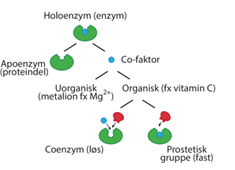
\includegraphics[width=0.8\textwidth]{figurs/enzym.png}
    \caption{Enzym}
    \label{fig:enzym}
\end{figure}
Enzymer er som sagt opbygget af proteiner, og måden disse proteiner bliver lavet er ved brug af en process der hedder det centrale dogme. Her bliver DNA lavet om til RNA som så bliver lavet om til protein. Det første trin i processen er transkription og det andet trin er translation. Under transkriptionen bliver DNA sekvensen analyseret og bliver omskrevet til hvad det vil svare til i en RNA sekvens ved brug af RNA-polymerase. Under translation bliver informationen på et mRNA-molekyle oversat til en rækkefølge af aminosyrer i et polypeptid ved brug af codonnets anticodon fra tRNA. Når der er dannet en lang kæde af aminosyrer bliver det så til et protein, som så kan bruges til at lave et enzym.
For at en reaktion kan foregå i kroppen skal to molekyler ramme hinanden hurtigt med en præcis vinke. Det lyder måske ikke så svært men man skal også huske at molekylerne ikke selv bestemmer hvordan de rejser rundt i blodet, da de ikke er levende. Dog kan det selvfølgeligt godt ske, dog er kravene til det meget svære at opnå uden ekstern hjælp. Det er der hvor enzymer kommer ind da de ”fanger” molekylerne og sikrer at de rammer hinanden med den rette orientering. Enzymet gør også så molekylerne ikke har brug for at have en høj nok bevægelsesenergi for at kunne reagere med hinanden og danne et nyt stof, uden et enzym ville man kunne øge bevægelsensenergien ved at øge temperaturen. Dog betyder det også at enzymer er meget specifikke og kan katalyserer en enkelt eller nogle få reaktioner. 
\begin{figure}
    \centering
    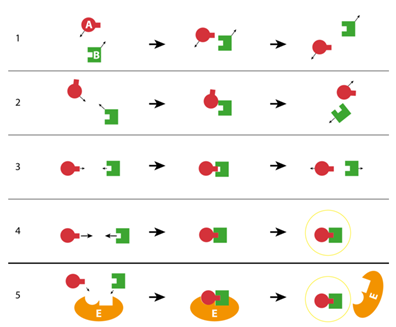
\includegraphics[width=0.8\textwidth]{figurs/enzym1.png}
    \caption{Enzym}
    \label{fig:enzym2}
\end{figure}
Det er faktisk ikke sindsygt svært at påvirke enzymer for enten det bedre eller det værre. Det kan man da enzymer virker bedst i specifikke miljøer og denaturer hvis miljøet er for ekstremt for dem. I øvelsen bromelin i ananas skulle vi klargøre en masse reagensglas med vand og opløst gelatine. I en af reagensglassene skulle vi tilsætte noget frisk ananasjuice fra en frisk presset ananas. Vi skulle også tilsætte konserveret ananassaft, ananasjuice og ananassaft fra dåse. I min gruppe puttede vi også saltsyre sammen med ananassaft for at se hvordan det daville påvirke gelatinens evne til at størkne. Formålet med øvelsen var at finde ud af hvornår et enzym, bromelin, ville hindre gelatine, som består af protein, i at størkne og danne gele. Vi gjorde det for at se om bromelin ville blive denatureret i forskellige miljø og hindre det i at virke. Her kunne vi tydeligt se hvor let det er at påvirke et enzym, for eksempel i reagensglasset med dåse ananas kunne vi se at der var der ingen reaktion mellem bromelinen og gelatinen. Det giver også god mening da dåsen formentligt er blevet varmebehandlet og derfor er bromelinen denatureret, da bromelinen er kommet i miljø der er alt for varmt og kommet over et point of no return. 
Der er mange konsekvenser ved mangel eller ændring af enzymer i en organisme, da hvis man mangler enzymer, kan nogle reaktioner ikke bliver katalyseret og derfor ikke finde sted i et stort nok omfang til at reaktionen er brugbar. En af de mere kendte sygdomme af mangel på et enzym er en tilstand kaldet laktoseintolerance. Her har personen ikke nok af enzymet laktase og vil derfor også have problemer med at nedbryde laktose. Ved ændring af enzymer i en organisme vil det samme nok også ske, dog kommer det selvfølgelig an på hvad det ændrer sig fra og hvad det ændrer sig til, dog er det nok typisk en dårlig ændring. Et eksempel på dette kan være at man har et enzym som katalyserer en livsnødvendig reaktion i kroppen, men så pludsligt af en ukendt årsag ændrer enzymet sig til noget andet som ikke kan katalyserer den samme reaktion. Det ville jo tydeligvis være meget dårligt da denne livsnødvendige reaktion ikke længere ville kunne foregå og organismen ville højest sandsynligt dø. 

    \newpage
\part{Proteinsyntese}
\subsection*{Forklar hvad DNA, kromosomer og gener er, samt hvordan de er opbygget.}
\subsection*{Redegør for hvordan der dannes protein ud fra gener.}
\subsection*{Med udgangspunkt i øvelsen: DNA fra løg, ønskes en diskussion af anvendelsen af DNA.}
DNA (de-oxy-ribo-nuclein-syre) er opbygget af nucleotider, som er sat sammen i lange kæder som kaldes polynucleotid-kæder.  Nucleotider består af tre forskellige dele: en phosphat gruppe, et kulhydrat og en nitrogenholdig base (Adenin, Guanin, Cytosin og Thymin). DNA er opbygget af to antiparallele strenge som snor sammen til at danne en dobbelthelix. Strengene bliver holdt sammen af hydrogenbindinger mellem de forskellige nitrogenholdige baser. Adenin med Thymin og Guanin med Cytosin. Dannelsen af en af strengene starter altid ved en phosphat gruppe på 5 mærke positionen i kulhydrat-ringen i det nukleotid hvor strengen bliver dannet, og slutter ved at blive bundet til stregen som vokser ved brug af OH (Hydroxid) gruppen som sidder på 3 mærke.
Kromosomer er struktuerer i cellerne lavet af DNA og proteiner. Dog er det DNA som er snoet rundt om proteiner, som kaldes histoner. Når DNA’et er snoet rundt om 8 histoner bliver der lavet en nukleosom, og når disse nukleosomer er pakket tæt bliver de kaldt kromosomer. Et menneske har normalt 46 kromosomer. 
Gener er opbygget af en af specifik sekvens af baser, som indeholder information, der fortæller cellen at den skal producere et protein baseret på sekvensen af baser. For at kunne lave proteinet skal cellen gøre flere ting, den skal kopierer DNA sekvensen til mRNA og derefter oversætte det til et protein ved brug af cellens ribosomer. De er ansvarlige for arvelighed og overførsel af træk fra ens forældre til en selv. Gener er unikke for hver organisme og bestemmer træk. 
Disse gener bliver brugt til at lave forskellige proteiner som bliver brugt rundt i kroppen. Processen for produktionen af DNA til protein bliver typisk kaldt Det centrale dogme. Processen siger at DNA bliver til RNA som bliver til protein. Første trin kaldes transkription og det andet trin kaldes translation.
Under transkription bliver længden af DNA sekvensen brugt til at bestemme hvor lang selve protein kæden kommer til at blive når hele processen er færdig. I denne fase bliver DNA sekvensen omskrevet til hvad det ville svare til i en RNA sekvensm ved hjælp af RNA-polymerase. RNA er meget ligesom DNA, da det også er lavet af en kæde nucleotider, som også er lavet af en phosphat-gruppe, et kulhydrat og fire forskellige baser. Dog har RNA ikke thymine ligesom normalt DNA, men i stedet uracil. Det betyder at i RNA vil alle steder hvor der havde vøret thymine i DNA bliver lavet om til uracil i RNAet. 
Under translation bliver informationen på et mRNA-molekyle oversat til en rækkefølge af aminosyrer i et polypeptid. 
Dog svarer en base ikke til en aminosyre, da der kun findes 20 forskellige aminosyrer og 4 forskellige baser. Man har brug for tre baser til at danne en animosyre og siden der er fire forskellige baser kan man sige \begin{math}4^3=64\end{math}. Det betyder at der er 64 forskellige kombinationer af baserne, men siden der kun er 20 forskellige aminosyrer, kan nogle af dem have flere forskellige codons. Ved eukaryoter starter polypeptid kæden nærmest altid med codonnet AUG eller methionin og ved prokaryoter er det typisk GUG eller valin. 
Polypeptid kæden ved at den er færdig når den kommer mod en af de tre stop-codons, UAA, UAG eller UGA.
Aflæsningen af mRNA og oversættelsen af codons til aminosyrer forgår på ribosomerne, som er organeller der flyder rundt i cellens cytoplasma. De kaldes også celles proteinfabrik. Genkendelsen af dem forgår på et specialiseret RNA-molekyle som kaldes tRNA (transfer RNA) og for hvert animosyre er der en specifik tRNA-molekyle. TRNA binder de specielle aminosyrer i en ende og indeholder et anitcodon i den anden ende. Et anticodon baseparrer med codonnet i mRNA. For eksempel vil et anticodon til GAG være CUC.
Til selve translation er der tre forskellige faser gennem processen. Initering, elongering og terminering
\begin{longtable}{| m{2cm} | m{7cm} | }
    \hline 
    Fase & Beskrivelse \\ \hline
    Initering & mRNA bindes til ribosomet og start-codonnet bliver fundet. Methionin tilføres til et anticodon typisk UAC ved hjælp af tRNA. \\ \hline
    Elongering & I denne fase bliver de rigtige aminosyrer tilført via tRNA. Anticodonnet genkender de forskellige codonner og binder til de rigtige i mRNA'et. Mellem de tilførte aminosyrer og tRNA molekylerne dannes peptidbindinger, og der bliver gjort klar til at transportere en aminosyre til en anden proteinfabrik- \\ \hline
    Terminering & I denne fase bliver stop-codonnet aflæst og den dannede polypeptidkæde bliver frigjort fra ribosomerne, og når denne polypeptidkæde bliver foldet rigtigt bliver den lavet om til et protein. \\ \hline
\end{longtable}
I forsøget DNA fra løg skulle vi isolere DNA'et fra et løg ved at først nedbryde vævet ved brug af en blender. Vi skulle også fjerne cellevægge, cellemembraner og kernemembraner ved brug af et vaskemiddel. Efter det skulle vi filtrerer alt ubrugeligt materiale ved at bruge et kaffefilter. Eftersom at der også var proteiner skulle vi også fjerne dem da vi kun var interreseret i DNA'et, for at fjerne proteinerne skulle vi bruge et protease enzym. Til sidst hældte vi iskold ethanol ned af siden af reagensglasset for at danne et lag af ethanol over løg-ekstraktet. 
Der er mange mulige anvendelser af udvundet DNA, nogle af dem jeg kan tænke på er at sekvensere DNA. Det er rimelig brugbart da det lader os finde ud af hvilke genetiske variationer øger farlige sygdomer og andre ting som man helst vil undgå. En anden anvendelse af udvundet DNA er at man kan analyserer planters DNA før de bliver planet for at se hvilke planter vil være bedre at plante og dermed foretage selektiv avl.

    \newpage
\part{Genetik}
\subsection*{Forklar hvad der forstås ved nedarvning, herunder 1-gen dominant/recessiv nedarvning.}
\subsection*{Redegør for mutationer, samt hvordan de kan lede til variation.}
\subsection*{Diskuter hvordan fænotyper kan have betydning for evnen til at overleve. Tag udgangspunkt i øvelse om selektion}
    \newpage
\section{Evolution}
\subsection{Forklar hvad der forstås ved evolution. Kom herunder ind på, hvad der driver evolution}
\subsection{Redegør for mutationer, samt hvordan de kan lede til variation. Inddrag gerne øvelse om selektion.}
\subsection{Med udgangspunkt i øvelsen om dykkerrefleks, ønskes en diskussion af udvikling af mekanismen, samt en diskussion om udviklingen af nye arter.}
    \newpage
\section{Kulstofkredsløb}
\subsection{Redegør for hvordan carbon/energi flyttes rundt i et kredsløb}
\subsection{Forklar processerne fotosyntese og respiration, herunder indragelse af øvelsen: Fotosyntese og respiration}
\subsection{Diskuter hvordan fotosyntese og respiration spiller en vigtig rolle for økosystemer og klimaet}
    \newpage
\section{DNA og kromosomer}
\subsection{Redegør for hvordan kromosomer og DNA er opbygget}
\subsection{Forklar de 2 celledelinger mitose og meiose og diskuter hvordan mutationer opstår}
\subsection{Redegør for øvelsen DNA fra løg og kom ind på mulig anvendelse af udvundet DNA}
    \newpage
\part{Bakteriel vækst}
\subsection*{Redegør for bakteriecellers opbygning}
\subsection*{Forklar den bakterielle vækstkurve og kom ind på typen af celledeling, samt hvad der sker i de enkelte faser. Diskuter formål og forskelle mellem mitose og meiose}
\subsection*{I forhold til forsøget om osmose skal det diskuteres hvordan salt mm, kan anvendes til konservering, samt hvilken effekt det kan have på bakterier såvel som større organismer.}
Bakterierceller er encellede prokaryote organismer som har en cellemembran og cellevæg omkring. Bakteriecellen er opbygget ligesom mange andre celler, en cellemembran lavet af phosplipider, forskellige typer proteiner inde i cellen, cytoplasma med en masse forskellige organeller som bakteriekromosomet, plasmider og ribosomer. 
Plasmiderne er meget små cirkulære stykker DNA-molekyler som kan kopiere sig selv. Der er cirka 40-60 af dem per bakteriecelle. Bakteriekromosomot er også i stand til at kopiere sig selv ligesom plasmiderne, de er omgivet af proteiner og flyder rundt frit i cytoplasmaet. Ved ribosomerne foregår proteinsyntese af enzymer til cellen, stofskifte eller proteiner. 
Bakterier bliver typisk opdelt i to grupper, Gramnegative og Grampositive. Grampositive bakterier har en cellevæg lavet af et tykt lag peptidoglycan, som er opbygget af N-acetylglucosamin og N-acetylmuraminsyre, hvor alt holdes sammen af oligopeptider. Cellevæggen bliver bundet sammen med cellemembranen af lipoteichoinsyre. Gramnegative bakterier har også en cellevæg, dog består den af et tyndt lag peptidoglycan og en ydre membran. Den ydre membran bliver holdt sammen med cellevæggen med lipopolysaccharider og lipoproteiner.
Mængden af bakterier vil ikke kune øge forevigt, men vil i stedet begynder at falde og ofte ende med at mange af bakterierne vil dø. Der er typisk fire faser i bakterievæksten, nølefasen, eksponentiel fasen, stationær fasen og dødsfasen. Bakterier går ikke igennem mitose eller meiose ligesom andre celler da det jo kun er eukaryote celler der går gennem de to typer celldelinger. Bakterier går gennem noget som kaldes binær fission hvor cellen bliver spaltet og laver datterceller. Formålet med denne type deling er bare at formere.

\begin{longtable}{| m{3cm} | m{14cm} |}
    Fase & Beskrivelse \\ \hline
    
    Nøglefase & I nølefasen stiger antallet af celler ikke, da bakterien stadig er i gang med at tilpasse sig til næringsmediet. Mængden af tid denne fase tager varier meget og viser behovet for produktion af nye enzymer som tillader bakteriet at udnytte næringsmediet. \\ \hline

    Eksponentiel fase &  I den eksponentielle vækstfase vil mængden af bakterier fordoble efter den samme mængde tid. Det betyder at hvis man startede med 20 bakterier og efter 5 min havde 40 bakterier så ville man vide at mængden af bakterier altid vil fordoble efter 5 min. \\ \hline

    Stationær fase &  I den stationære fase vil mængden af bakterier ikke stige, da mængden af nye bakterier modsvares af mængden af bakterier. \\  \hline 

    Dødsfase & I dødsfasen vil mængden af bakterier der dør bliver større end mængden af nye baktierer hvilket betyder at mængden af totalle bakterier vil falde. \\ \hline

\end{longtable}

Mitose og meiose er de to forskellige måder en celle kan dele sig. Dog er det ikke tilfældigt hvilken af de to måder cellen kommer til at dele sig på. Hvis cellen er en kønscelle vil den gå igennem meiose for at dele sig og hvis cellen ikke er en kønscelle vil den gå gennem mitose for at dele sig.
I mitosen er der fem forskellige faser som en celle går igennem før den bliver delt og har lavet flere celler. Interfasen, profasen, metafasen, anafasen og telofasen. Formålet for mitosen er fomering, vækst og vedligeholdelse.

\begin{longtable}{| m{3cm} | m{14cm} |}
    \hline 
    Fase & Beskrivelse \\ \hline
    Interfasen & Interfasen er den fase som cellen bruger det meste af tiden i, da det er den fase hvor cellen bare laver de normalle ting en celle gør. Dog når cellen kommer tættere på at dele sig selv begynder DNA-strengene (kromatin) at strække sig ud, centrosomer og DNA begynder også at kopierer sig selv. \\ \hline

    Profasen & I profasen begynder kromatinet at kondensere og begynder at ligne kromosomer. Disse kromosomer består af to identiske søsterkromatider, som er forbundet i midten ved et centromer. Cellekernen, som indeholder alt af en celles DNA, begynder også at blive nedbrudt i denne fase og centrosomerne flytter sig hen til forskellige sider af cellen \\ \hline

    Metafasen & I metafasen, nu hvor kromosomerne er fuldt kondenseret, begynder kromosomerne at flytte sig ind til midten af cellen, for at danne en lige linje. De danner en lige linje for at sikre sig at søsterkromatiderne kan blive skilt ordenligt i den næste fase af mitosen. \\ \hline

    Anafasen & Under anafasen bliver kromosomerne skilt og de to søsterkromatider som kromosomerne bestod af bliver trukket til hver ende af cellen. Selve cellen begynder også at strække sig og cellen bliver tættere på at dele sig helt. \\ \hline

    Telofasen & Under telofasen bliver selve cellen splittet og bliver lavet om til to identiske datterceller. Kromosomerne begynder også at returnere til deres tidligere form som kromatin og forskellige organeller i cellen, ligesom cellekernen, begynder at blive genformet. \\ \hline
    
\end{longtable}

Meiosen er en måde at en celle kan dele sig, dog er det kun kønsceller eller gameter, som går igennem meiosen. Der er ni faser i meiosen, som er interfasen, profasen I, metafasen I, anafasen I, telofasen I, profasen II, metafasen II, anafasen II og telofasen II. Formålet med meiose er at danne kønsceller i forbindelse med kønnet formering.
\begin{longtable}{ | m{3cm} | m{14cm} |}
    \caption{Meiose} \\
    \hline
    Fase & Beskrivelse \\ \hline
    
    Interfase & Interfasen under meiose er præcist den samme som under mitosen. Cellen begynder at kopierer dens DNA og  gør sig klar til at begynde processen. \\ \hline

    Profase & Den første gang cellen går igennem profasen ligner fasen meget profasen i mitose, da kromatinet begynder at kondensere og begynder også at ligne kromosomer. Dog bliver kromosomernes genetiske materiale udvekles med andre kromosomer. Det gør så cellen opår genetisk variation. \\ \hline

    Metafase &  I den første metafase blier kromosomerne arrageret i par og bliver fastgjort til spindelapparatet for at gøre dem klar til at blive trukket til begge sider af cellen. \\ \hline

    Anafase & I anafase I bliver kromosomparrene delt og trukket til begge sider. Dog ligesom i mitosen bliver kromosomerne skilt og de to kromatider som kromosomerne bestod af bliver også trukket til hver side af cellen. \\ \hline

    Telofase & I telofase I bliver cellerne delt helt, hvilket betyder at der nu er to datterceller som er haploide, hvilket betyder at deres kromosomantal er halveret. Nye cellekerne bliver også dannet og kromosomerne begynder at dekondensere. \\ \hline

   Profase II & Igen i profase II begynder kromosomerne at blive kondenseret og cellekernet bliver også nedbrudt igen. Centriolerne begynder også at flytte sig hen til modsatte sider af cellen for at gøre klar til de næste faser. \\ \hline
 
    Metafase II &  Kromosomerne begynder at bevæge sig ind mod midten af cellen i en lige linje og kromosomerne gør sig klar til at blive adskilt i den næste fase. \\ \hline

    Anafase II & Kromosomerne begynder at bevæge sig ind mod midten af cellen i en lige linje og kromosomerne gør sig klar til at blive adskilt i den næste fase. \\ \hline

    Telofase II & I telofase II bliver cellerne delt igen hvilket betyder at der nu er fire celler til sidst. Nye cellekerne bliver også genbygget inde i cellerne for at holde på en celles DNA. Kromosomerne dekondenserer også igen og meiosen er færdig efter dette trin. \\ \hline

\end{longtable}

\begin{longtable}{ | m{5cm} | m{5cm} | m{5cm} | }
    \hline 
    & Meiose & Mitose \\ \hline
    Genetisk variation & Ja & Nej \\ \hline
    Antal datterceller & 4 & 2 \\ \hline
    Type celle & kønsceller & Somatiske celler \\ \hline
    mængde divisioner & 2 & 1 \\ \hline
\end{longtable}

I forsøget om osmotisk salinitet skulle vi putte lige store stykker kartofler ind i reagensglas med vand med forskellige koncentrationer af salt. Vi fandt ud af når kartoflen kom ind i et hypotonisk miljø altså et miljø med højere vandkonkenctration end inde i kartoflen ville massen af kartoflen stige, da vandet vil bevæge sig ind i cellerne. Vi fandt også ud af når kartoflen var i et hypertonisk miljø, altså et miljø hvor koncentrationen af ikke flytbart stof er højere end inde i kartoflen, ville massen af kartoflen formindske, da vandet vil bevæge sig ud af cellerne.
Salt kan derfor godt blive brugt som et konserveringsmiddel da ved brug af osmose vil det danne et hypertonisk miljø. Et miljø hvor stofkoncentrationen er højere udenfor cellerne end inde i cellerne, og vandet vil trænge gennem en semipermeabel membran for at udligne miljøet og opnå et isotonisk miljø. Salt virker derfor godt da det vil få vandet i bakterier til at gå gennem membranen og derfor også dræbe bakterien, da de har brug for vand til at trive. Salt vil også stoppe mug og skimmelsvamp da det også mængden af vand inde i cellerne vil falde. Det betyder at mad vil kunne være spiseligt i meget længere tid.

    \input{chapters/99Bilag.tex}
    %\bibliography{sources/library}
\end{document}